\problem{1: PortKnock Firewall}{6}
Implement a port-knock firewall which drops all packets from an IP source until the secret right sequence of TCP port numbers \{2222,3333,4444\} is knocked. When the right sequence is knocked, the bmv2 switch must forward out of one of its ports the next TCP packets with destination port 22 from the same IP source.\\
To test the behavior of your program we provide you with two python scripts running a client and a server for this application. The \textit{portKnocker.py} script can generate both the right sequence of ports and sequences of random ports based different input parameters. The \textit{knockedServer.py} simply listens to a specific virtual interface the bmv2 switch is connected to and prints out the packets forwarded out of that interface by the switch.\\
~\\
The following steps illustrate a typical workflow to work on this task:
\begin{enumerate}
\item Unzip to a folder the portKnockFirewall archive:\\
       \textit{ \$: unzip problem1.zip} 
\item Edit the template of the main program:\\
        \textit{\$: vim main.p4}
\item Iteratively compile and fix your P4 code:\\
       \textit{ \$: p4c-bm2-ss --arch v1model main.p4 -o main.json}
\item Create some veth interfaces and start the bmv2 switch:\\
        \textit{\$: sudo veth\_setup.sh}\\
        \textit{\$: sudo simple\_switch -i 0@veth0 -i 1@veth4 --log-console \$FULL\_PATH\_TO\_YOUR/main.json}
\item Write down your table entries into a text file, e.g., "\textit{commands.txt}", and populate the switch's tables:\\
        %\textit{\$: runtime\_CLI $<$ commands.txt}
        \textit{\$: python /usr/local/lib/python2.7/dist-packages/runtime\_CLI.py $<$ commands.txt}
\item Test your program as illustrated by the following image: i) 0pen a terminal and start the server script, ii) 0pen a different terminal and try first with a wrong sequence of port numbers and then iii) with the right one. In the former case, you should see no packets printed by the server, while in latter the server should print the ssh packets forwarded out by the switch.
\end{enumerate}

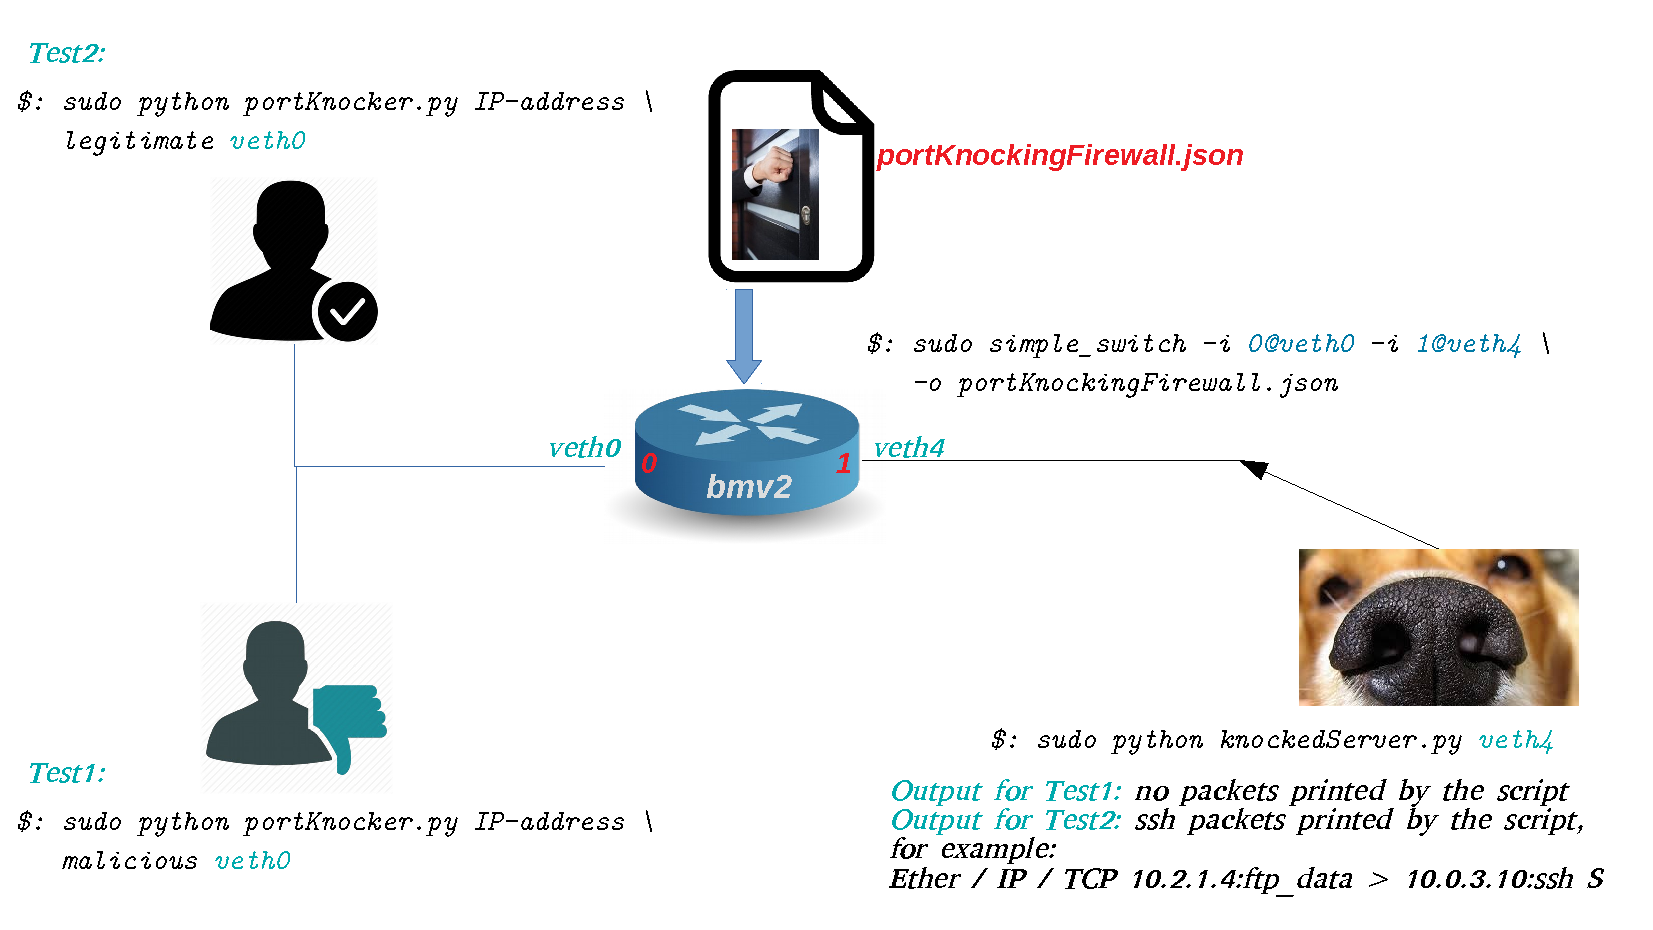
\includegraphics[width=1\textwidth]{./images/testPortKnockFw.pdf}
~\\
\subproblem{Submission} We expect you to deliver a P4 program (p4 source files and table entries) which we can load into the switch and test by using the same two python scripts provided to you.